% Provenance (never printed): see sources/outline_sources.md (Year 1: hotspots and
% mantle plumes; hotspot chains and absolute plate motion; large igneous provinces).
% Hotspot map, pole fit, rates and swell from figdata/bachelor-1/hotspots.py (data
% data/derived/bachelor-1-hotspots.csv, Table 1 of the Morgan and Morgan 2007 electronic
% supplement); exercise and problem values in the Book 3 scratch calculators calc/ch15.py and
% calc/ch15ex.py. "Hotspot" is re-founded from Book 1 (g7 volcanoes), "hotspot track"
% from Book 2 (g11 plate-motions); Book 2 owns the age--distance fit of the Hawaiian
% chain, so this chapter fits the Pacific Euler pole from track directions instead.
\chapter{हॉटस्पॉट और अंतःप्लेट ज्वालामुखी}\label{ch:b1:hotspots}

जनवरी 1983 से, और उसके बाद दशकों तक, हवाई द्वीप के किलाउआ ने अपने पूर्वी दरार-क्षेत्र के एक छिद्र, Pu\textquoteleft u~\textquoteleft O\textquoteleft o, से लगभग बिना रुके उद्गार किए, और प्रति वर्ष लगभग \qty{0.12}{km^3} लावा निकाला। किलाउआ प्रशांत प्लेट के मध्य में खड़ा है, किसी कटक या खाई से हज़ारों किलोमीटर दूर। उत्तर-पश्चिम की ओर हवाई के द्वीप अधिकाधिक पुराने होते जाते हैं, फिर वे समुद्र में डूब जाते हैं और शृंखला हज़ारों किलोमीटर और तक डूबे हुए ज्वालामुखियों की एक रेखा के रूप में चलती रहती है।
प्लेट विवर्तनिकी प्लेट-सीमाओं पर के ज्वालामुखियों को समझाती है; यह अध्याय उन ज्वालामुखियों के बारे में है जिन्हें वह सीधे नहीं समझाती, यानी \omterm{def:b1:hotspots:hotspot}{हॉटस्पॉट}, और इस बदले में वे हमें क्या बताते हैं: प्लेटें गहरे \omterm{def:b1:layered-earth:layers}{प्रावार} पर कैसे चलती हैं, नीचे से कितनी ऊष्मा और चट्टान ऊपर उठती है, और कैसे कुछ विशाल लावा-उद्गार, यानी \omterm{def:b1:hotspots:lip}{बृहत आग्नेय प्रांत}, बने।
% ledger: pp1801:kilauea-rate

\begin{recall}
एक \omterm{def:b1:hotspots:hotspot}{हॉटस्पॉट} प्लेट के ऊपर से गुज़रते समय गहरे \omterm{def:b1:layered-earth:layers}{प्रावार} से ज्वालामुखियों को पोषित करता है, और प्लेट एक \omterm{def:b1:hotspots:track}{हॉटस्पॉट-पथ} ढो ले जाती है जिसके ज्वालामुखी दूरी के साथ अधिक पुराने होते हैं (पुस्तक 1, कक्षा 7; पुस्तक 2, कक्षा 11)। \omterm{def:b1:plate-kinematics:euler-pole}{यूलर सदिश} $\vec\omega$ के साथ घूमती प्लेट $\vec v = \vec\omega\times\vec r$ के अनुसार चलती है, $\omega R\sin\Delta$ की चाल से, उस \omterm{def:b1:spherical-astronomy:spherical-triangle}{महावृत्त} के लंबवत जो उसे ध्रुव से जोड़ता है (\cref{ch:b1:plate-kinematics}); उभार \omterm{def:b1:isostasy-gravity:isostasy}{समस्थिति} से टिका रहता है (\cref{ch:b1:isostasy-gravity}); गरम चट्टान $\alpha\,\Delta T$ अंश से हल्की होती है (\cref{ch:b1:rifts-ridges-margins})।
\end{recall}

\section{हॉटस्पॉट और प्रावार-स्तंभ}\label{sec:b1:hotspots:plumes}

\begin{definition}[हॉटस्पॉट]
\label{def:b1:hotspots:hotspot}
एक \emph{हॉटस्पॉट}\index{हॉटस्पॉट} ज्वालामुखीय-क्रियाकलाप का वह क्षेत्र है जिसकी स्थिति प्लेट-सीमाओं पर निर्भर नहीं करती, जो दसियों मिलियन वर्षों तक सक्रिय रहता है, और जिसे उसके आसपास के \omterm{def:b1:layered-earth:layers}{प्रावार} से गरम \omterm{def:b1:layered-earth:layers}{प्रावार} से पोषित माना जाता है।
\end{definition}

कितने \omterm{def:b1:hotspots:hotspot}{हॉटस्पॉट} हैं, यह इस पर निर्भर करता है कि कौन गिनता है। इस अध्याय में प्रयुक्त हॉटस्पॉट-सारणी उनमें 68 सूचीबद्ध करती है, पर उसके लेखक कई ऐसी विशेषताएँ छोड़ देते हैं जिन्हें वे प्लेट की गति दर्ज करने वाली नहीं मानते, और उनमें से कुछ को, जिन्हें वे रखते हैं, केवल संभावित मानकर चलते हैं। कुछ \omterm{def:b1:hotspots:hotspot}{हॉटस्पॉट}, जिनमें हवाई, आइसलैंड और रेयूनियन हैं, लंबे, नियमित पथ और बड़ा उत्पादन रखते हैं, जैसा किसी गहरे स्रोत से अपेक्षित है; दूसरे छोटे और अल्पकालिक हैं। अधिकांश हॉटस्पॉट-ज्वालामुखी बेसाल्ट उगलते हैं; जहाँ कोई \omterm{def:b1:hotspots:hotspot}{हॉटस्पॉट} महाद्वीप के नीचे हो, वहाँ गरम बेसाल्ट \omterm{def:b1:layered-earth:layers}{भूपर्पटी} को पिघलाता है, और बड़े उद्गार राइओलाइट में बदल जाते हैं, जैसे येलोस्टोन में।
% ledger: mm07:table, data:b3-hotspots, yvo:calderas

\begin{definition}[प्रावार-स्तंभ]
\label{def:b1:hotspots:plume}
एक \emph{प्रावार-स्तंभ}\index{प्रावार-स्तंभ} गरम, उत्प्लावी प्रावार-चट्टान का एक स्तंभ है जो \omterm{def:b1:layered-earth:layers}{प्रावार} के भीतर गहरे एक \omterm{def:b1:heat-budget:boundary-layer}{ऊष्मीय सीमा-परत} से उठता है। नए स्तंभ का एक बड़ा, गोलाकार \emph{शीर्ष} होता है जो एक लंबी, पतली \emph{पुच्छ}, या नली, पर टिका होता है; एक बार शीर्ष \omterm{def:b1:layered-earth:lithosphere}{स्थलमंडल} के नीचे फैल जाए, तो पुच्छ दसियों मिलियन वर्षों तक सतह तक पिघला पदार्थ पहुँचाती रहती है।
\end{definition}

यह आकार प्रयोगशाला से आता है। 1970 के दशक के टंकी-प्रयोगों में, ऊपर के द्रव से कम श्यान हल्के द्रव की एक परत एक गोल पॉकेट के रूप में ऊपर उठी, जिसे पीछे की एक नली से पोषण मिलता था: एक मशरूम। \omterm{def:b1:layered-earth:lithosphere}{स्थलमंडल} के आधार तक पहुँचता \omterm{def:b1:hotspots:plume}{प्रावार-स्तंभ} का शीर्ष फैलकर चपटा हो जाता है; दाब घटता है, और गरम चट्टान बड़ी मात्रा में पिघलती है। बाढ़-बेसाल्ट इस चित्र में बैठते हैं: उनका ज्वालामुखी-क्रियाकलाप लगभग दस मिलियन वर्ष चलता है, पर उनके अधिकांश आयतन का उद्गार लगभग दस लाख वर्ष या उससे कम में होता है, और वे अक्सर किसी महाद्वीप के टूटने के साथ आते हैं (\cref{sec:b1:hotspots:lips})।
% ledger: hist:plumes (Whitehead and Luther 1975), cr03:summary

\begin{omfigure}
\begin{tikzpicture}[font=\scriptsize,
  lbl/.style={fill=white, fill opacity=0.8, text opacity=1, inner sep=1pt, align=center}]
% ---- panel (a): the head arrives ----
\begin{scope}
\clip (0,-5) rectangle (6.4,1.3);
\fill[orange!12] (0,-5) rectangle (6.4,0);
\fill[omSea!45] (0,0) rectangle (6.4,0.55);
\fill[omLithBasalt!55] (0,0) rectangle (6.4,-0.9);
% flood basalt: a stack of flat flows on the sea floor
\fill[black!55] (2.5,0) -- (2.7,0.32) -- (6.1,0.32) -- (6.3,0) -- cycle;
\foreach \y in {0.08,0.16,0.24} \draw[white!70!black, line width=0.3pt] (2.62,\y) -- (6.18,\y);
% plume: tail and flattened head
\fill[red!40] (4.25,-5) -- (4.25,-1.7) -- (4.55,-1.7) -- (4.55,-5) -- cycle;
\fill[red!40] (4.4,-1.45) ellipse[x radius=1.9, y radius=0.55];
\draw[red!60!black, line width=0.4pt] (4.25,-5) -- (4.25,-1.95) (4.55,-5) -- (4.55,-1.95);
\draw[red!60!black, line width=0.4pt] (4.4,-1.45) ellipse[x radius=1.9, y radius=0.55];
% melt rising through the plate
\foreach \x in {3.2,3.9,4.6,5.3}
  \draw[red!75!black, line width=0.6pt, decorate, decoration={snake, amplitude=0.6pt, segment length=3pt}] (\x,-1.1) -- (\x,0.05);
\end{scope}
\draw[black!70] (0,-5) rectangle (6.4,1.3);
\node[lbl, anchor=north west] at (0.1,1.25) {(क) शीर्ष पहुँचता है};
\node[lbl, anchor=west] at (0.1,-0.45) {स्थलमंडल};
\node[lbl, anchor=west] at (0.1,0.3) {समुद्र};
\node[lbl, anchor=south] at (4.4,0.62) {बाढ़-बेसाल्ट (LIP)};
\node[lbl, anchor=east] (ph) at (1.9,-1.75) {स्तंभ-शीर्ष};
\draw[black!70] (ph.east) -- (2.7,-1.6);
\node[lbl, anchor=east] at (4.1,-3.6) {स्तंभ-पुच्छ};
\node[lbl, anchor=west] at (0.1,-4.6) {प्रावार};
% ---- panel (b): the plate has moved on ----
\begin{scope}[xshift=6.8cm]
\begin{scope}
\clip (0,-5) rectangle (6.4,1.3);
\fill[orange!12] (0,-5) rectangle (6.4,0);
\fill[omSea!45] (0,0) rectangle (6.4,0.55);
\fill[omLithBasalt!55] (0,0) rectangle (6.4,-0.9);
% the flood basalt, carried away to the left
\fill[black!55] (-0.9,0) -- (-0.7,0.32) -- (1.0,0.32) -- (1.2,0) -- cycle;
\foreach \y in {0.08,0.16,0.24} \draw[white!70!black, line width=0.3pt] (-0.8,\y) -- (1.08,\y);
% the chain: older volcanoes to the left, lower (they sank as the plate cooled)
\fill[black!35] (1.45,0) -- (1.75,0.2) -- (2.05,0) -- cycle;
\fill[black!38] (2.15,0) -- (2.5,0.3) -- (2.85,0) -- cycle;
\fill[black!42] (2.95,0) -- (3.35,0.42) -- (3.75,0) -- cycle;
\fill[black!65] (3.95,0) -- (4.45,0.95) -- (4.55,0.97) -- (5.05,0) -- cycle;
\fill[red!70!black] (4.43,0.93) -- (4.57,0.95) -- (4.5,1.12) -- cycle;
% the plume tail, still in place, and a small spread of hot rock under the plate
\fill[red!40] (4.35,-5) -- (4.35,-1.1) -- (4.65,-1.1) -- (4.65,-5) -- cycle;
\fill[red!40] (4.5,-1.05) ellipse[x radius=0.75, y radius=0.2];
\draw[red!60!black, line width=0.4pt] (4.35,-5) -- (4.35,-1.2) (4.65,-5) -- (4.65,-1.2);
\draw[red!75!black, line width=0.6pt, decorate, decoration={snake, amplitude=0.6pt, segment length=3pt}] (4.5,-0.95) -- (4.5,0.8);
\end{scope}
\draw[black!70] (0,-5) rectangle (6.4,1.3);
\node[lbl, anchor=north west] at (0.1,1.25) {(ख) बहुत बाद में};
\draw[->, line width=1pt] (3.2,-0.45) -- (1.2,-0.45) node[midway, above=1pt, lbl] {प्लेट-गति};
\node[lbl, anchor=south] at (0.55,0.38) {LIP};
\node[lbl, anchor=south] at (2.7,0.62) {पुराना, सुप्त};
\node[lbl, anchor=west] at (5.0,0.95) {सक्रिय\\ज्वालामुखी};
\node[lbl, anchor=east] at (4.2,-3.6) {स्तंभ-पुच्छ};
\node[lbl, anchor=west] at (4.75,-2.6) {प्रावार में\\रुका रहता है};
\end{scope}
\end{tikzpicture}
\par\smallskip{\small \omterm{def:b1:hotspots:hotspot}{हॉटस्पॉट} का \omterm{def:b1:hotspots:plume}{प्रावार-स्तंभ} मॉडल (योजनाबद्ध, पैमाने पर नहीं)।
(क)~एक नया स्तंभ: उसका शीर्ष \omterm{def:b1:layered-earth:lithosphere}{स्थलमंडल} के नीचे चपटा होता है और दाब घटने के साथ पिघलता है, और एक बाढ़-बेसाल्ट, यानी एक \omterm{def:b1:hotspots:lip}{बृहत आग्नेय प्रांत},
कुछ मिलियन वर्षों या उससे कम में उगला जाता है। (ख)~दसियों मिलियन वर्ष बाद प्लेट उस प्रांत को दूर ले जा चुकी होती है; संकरी पुच्छ अब भी एक सक्रिय
ज्वालामुखी को पोषित करती है, और उससे पहले बने ज्वालामुखी सुप्त हैं, दूरी के साथ अधिक पुराने, और नीचे, क्योंकि वे ठंडी होती प्लेट के साथ धँसते हैं।}
\label{fig:b1:hotspots:plume}
\end{omfigure}

प्रावार-स्तंभों के पक्ष में क्या प्रमाण है? पहला, \omterm{def:b1:hotspots:track}{आयु-प्रगति} वाली शृंखलाएँ स्वयं, जिन्हें चलती प्लेट के नीचे स्थिर एक संकरा स्रोत तुरंत समझा देता है (\cref{sec:b1:hotspots:tracks})। दूसरा, कुछ हॉटस्पॉटों के लावा में हीलियम के हल्के और भारी समस्थानिक का असामान्य रूप से ऊँचा अनुपात होता है, जिसे एक गहरे भंडार का चिह्न माना जाता है, जिसने पृथ्वी के बनने के समय की कुछ गैस बचा रखी है। तीसरा, स्रोत गरम हैं: महासागरीय द्वीपों और पठारों के लावा \omterm{def:b1:layered-earth:layers}{प्रावार} की ओर इशारा करते हैं जो कटकों के नीचे के \omterm{def:b1:layered-earth:layers}{प्रावार} से 200 से \qty{300}{\celsius} अधिक गरम है, जिसका विभव-तापमान 1280 और \qty{1400}{\celsius} के बीच है। चौथा, \omterm{def:b1:layered-earth:layers}{प्रावार} के भूकंपीय चित्र: हवाई के नीचे, समुद्र-तल और द्वीपों पर भूकंपमापियों के एक जाल ने एक गरम स्तंभ को निचले \omterm{def:b1:layered-earth:layers}{प्रावार} तक नीचे जाते हुए चित्रित किया, और 2015 में पूर्ण भूकंपीय तरंग-रूपों से बने पूरे \omterm{def:b1:layered-earth:layers}{प्रावार} के एक प्रतिरूप में कई प्रमुख हॉटस्पॉटों के नीचे चौड़े, लगभग ऊर्ध्वाधर स्तंभ दिखते हैं, जो \omterm{def:b1:layered-earth:discontinuity}{कोर–प्रावार सीमा} से सतह के नीचे लगभग \qty{1000}{km} तक उठते हैं; हवाई, आइसलैंड और सामोआ के नीचे वे \omterm{def:b1:layered-earth:layers}{प्रावार} के आधार पर बहुत कम तरंग-गति वाले धब्बों में जड़े हैं। ऐसे चित्र कैसे बनते हैं, यह पुस्तक 5 का विषय है।
% ledger: herzberg:tp, wolfe:hawaii, fr15:plumes

इनमें से कुछ भी प्रमाण नहीं है, और बहस जीवित है। प्लेट-परिकल्पना में, जिसका समर्थन अन्य लोगों के साथ गिलियन फ़ाउल्जर और जेम्स नैटलैंड करते हैं, हॉटस्पॉट-ज्वालामुखी-क्रियाकलाप विशेष रूप से गरम नहीं होता और उसे गहरे स्तंभ की आवश्यकता नहीं: वह प्लेट विवर्तनिकी का एक उपोत्पाद है, जो उथले स्रोतों से पोषित होता है जहाँ \omterm{def:b1:layered-earth:lithosphere}{स्थलमंडल} खिंचा या दरका हुआ है। उनके विरोधी मानते हैं कि कम से कम कुछ गहरे स्तंभों के पक्ष में प्रमाण प्रबल है, यद्यपि भूकंपीय चित्र उसे तय करने जितने तीखे नहीं हैं; और \omterm{def:b1:hotspots:hotspot}{हॉटस्पॉट}, जैसा अगला खंड दिखाता है, पूरी तरह स्थिर नहीं हैं।
% ledger: fn03:plate-hypothesis, tarduno:emperor

\section{हॉटस्पॉट-पथ और प्लेटों की गति}\label{sec:b1:hotspots:tracks}

\begin{definition}[हॉटस्पॉट-पथ; आयु-प्रगति]
\label{def:b1:hotspots:track}
एक \emph{हॉटस्पॉट-पथ}\index{हॉटस्पॉट-पथ} ज्वालामुखियों, समुद्री पर्वतों और ज्वालामुखी कटकों की वह रेखा है जिसे प्लेट, \omterm{def:b1:hotspots:hotspot}{हॉटस्पॉट} के ऊपर से गुज़रते हुए, उससे दूर ले जाती है। उसकी \emph{आयु-प्रगति}\index{आयु-प्रगति} सक्रिय ज्वालामुखी से दूरी के साथ उसके ज्वालामुखियों की आयुओं की नियमित वृद्धि है। \omterm{def:b1:hotspots:hotspot}{हॉटस्पॉट} पर एक पथ की \emph{दिशा} वह दिगंश है, उत्तर से मापा गया, जिस ओर उसका तरुण भाग \omterm{def:b1:hotspots:hotspot}{हॉटस्पॉट} से दूर भागता है।
\end{definition}

यदि \omterm{def:b1:hotspots:hotspot}{हॉटस्पॉट} गहरे \omterm{def:b1:layered-earth:layers}{प्रावार} में स्थिर रहें, तो एक पथ गहरे \omterm{def:b1:layered-earth:layers}{प्रावार} के ऊपर प्लेट की गति दर्ज करता है: उसकी दिशा \omterm{def:b1:hotspots:hotspot}{हॉटस्पॉट} पर प्लेट के वेग की दिशा है, और उसकी \omterm{def:b1:hotspots:track}{आयु-प्रगति} चाल देती है। पुस्तक 2, कक्षा 11 ने हवाई के ज्वालामुखियों की आयुओं से प्रशांत प्लेट की चाल पढ़ी थी। केवल दिशाएँ ही इससे अधिक बताती हैं: वे \omterm{def:b1:plate-kinematics:euler-pole}{यूलर ध्रुव} देती हैं।

\begin{proposition}[दो पथों से यूलर ध्रुव]
\label{prop:b1:hotspots:two-tracks}
मान लीजिए एक \omterm{def:b1:plate-kinematics:rigid-plate}{दृढ़ प्लेट} दो स्थिर हॉटस्पॉटों पर, स्थितियों $\vec r_1$ और $\vec r_2$ पर, के ऊपर से चलती है, और मान लीजिए $\vec t_1$ और $\vec t_2$ उनके पथों के अनुदिश क्षैतिज इकाई सदिश हैं। यदि $\vec t_1$ और $\vec t_2$ समांतर नहीं हैं, तो हॉटस्पॉटों के सापेक्ष प्लेट का \omterm{def:b1:plate-kinematics:euler-pole}{यूलर सदिश} $\vec t_1\times\vec t_2$ के समांतर है, और उसका ध्रुव वह इकाई सदिश है
\[
  \vec p = \pm\frac{\vec t_1\times\vec t_2}{\lVert\vec t_1\times\vec t_2\rVert},
\]
चिह्न उसका है जिसके लिए $(\vec p\times\vec r_1)\cdot\vec t_1 > 0$।
\end{proposition}

\begin{proof}
हर \omterm{def:b1:hotspots:hotspot}{हॉटस्पॉट} पर प्लेट $\vec v_i = \vec\omega\times\vec r_i$ के साथ चलती है (\cref{thm:b1:plate-kinematics:velocity}), और पथ उसके अनुदिश इंगित करता है: $\vec v_i = v_i\vec t_i$ जहाँ $v_i > 0$। एक सदिश गुणनफल अपने गुणकों के लंबवत होता है, अतः $\vec\omega\cdot\vec t_i = 0$ होता है, $i = 1, 2$ के लिए: $\vec\omega$ दो ऐसे सदिशों के लंबवत है जो समांतर नहीं हैं, अतः वह उनके सदिश गुणनफल के समांतर है। उस पर के दो इकाई सदिशों में से ध्रुव वह है जिसके परितः घूर्णन वामावर्त है, यानी वह जिसके लिए $\vec p\times\vec r_1$ उस दिशा में इंगित करता है जिधर प्लेट पहले \omterm{def:b1:hotspots:hotspot}{हॉटस्पॉट} पर चलती है, अर्थात् $+\vec t_1$ की ओर।
\end{proof}

प्रस्ताव के प्रयोग के लिए, \omterm{def:b1:spherical-astronomy:geographic}{अक्षांश} $\varphi$ और \omterm{def:b1:spherical-astronomy:geographic}{देशांतर} $\lambda$ वाले एक बिंदु पर, पूर्व और उत्तर की ओर इंगित करने वाले इकाई सदिशों की आवश्यकता होती है,
\[
  \vec e = (-\sin\lambda,\ \cos\lambda,\ 0),\qquad
  \vec n = (-\sin\varphi\cos\lambda,\ -\sin\varphi\sin\lambda,\ \cos\varphi),
\]
(\cref{ch:b1:plate-kinematics}) के अक्षों में ($x$ की ओर \ang{0}\,N \ang{0}\,E, $y$ की ओर \ang{0}\,N \ang{90}\,E, $z$ उत्तरी ध्रुव की ओर)। दिगंश $\theta$ का एक पथ $\vec t = \sin\theta\,\vec e +
\cos\theta\,\vec n$ के अनुदिश चलता है। हवाई पथ, दिगंश \ang{304}, और लुईसविल पथ, दिगंश \ang{316}, के साथ यह प्रस्ताव प्रशांत प्लेट का ध्रुव \ang{56.2}\,S, \ang{124.0}\,E पर रखता है (सप्ताहांत समस्या में परिकलन किया गया है)।
% values (hotspots.py): two_pole_lat -56.1805, two_pole_lon 124.008; ledger: data:b3-hotspots

दो पथ ध्रुव तय करते हैं, पर उसकी परीक्षा नहीं कर सकते। कई पथ उसे अति-निर्धारित करते हैं, और विचलन बताता है कि \omterm{def:b1:hotspots:hotspot}{हॉटस्पॉट} एक स्थिर चौखटे की तरह व्यवहार करते हैं या नहीं। डब्ल्यू॰ जेसन मॉर्गन, जिन्होंने गहरे स्तंभों का प्रस्ताव रखा, और जेसन फ़िप्स मॉर्गन ने 2007 में 68 हॉटस्पॉटों की एक सारणी संकलित की, जिसमें, जहाँ वे मापे जा सकते थे, पथ की दिशा और \omterm{def:b1:hotspots:hotspot}{हॉटस्पॉट} पर प्लेट की चाल थी, हर एक अपनी अनिश्चितता और अपनी विश्वसनीयता के भार के साथ; आइसलैंड की तरह, जो दो प्लेटों के नीचे है, उसकी प्रत्येक प्लेट के लिए एक पंक्ति है। प्रशांत प्लेट पर पंद्रह भारित पथ पड़ते हैं, जिनमें से तेरह की चाल दी गई है।
% ledger: data:b3-hotspots, mm07:table; values (hotspots.py): n_all 71 rows, n_pacific 15, n_rated 13

\begin{method}[हॉटस्पॉट-पथों से यूलर ध्रुव और दर का अनुमान]
\label{met:b1:hotspots:pole-fit}
एक प्लेट पर $N$ हॉटस्पॉटों के लिए, उनकी स्थितियाँ, पथ-दिशाएँ $\theta_i \pm \sigma_i$ भारों $w_i$ के साथ, और उनमें से कुछ के लिए चालें $v_i$ दी गई हों:
\begin{enumerate}
  \item एक परीक्षण ध्रुव $\vec p$ के लिए, हर \omterm{def:b1:hotspots:hotspot}{हॉटस्पॉट} पर $\vec p\times\vec r_i$ की दिशा परिकलित कीजिए, और उससे अनुमानित गति का दिगंश $\hat\theta_i$ (\cref{prop:b1:plate-kinematics:speed})।
  \item विचलन $S(\vec p) = \sum_i w_i\bigl((\hat\theta_i -
        \theta_i)/\sigma_i\bigr)^2$ बनाइए, हर अंतर को \ang{-180} और \ang{180} के बीच लाकर।
  \item $S$ को न्यूनतम करने वाला ध्रुव खोजिए: पूरे गोले के एक ग्रिड पर, फिर सर्वोत्तम बिंदु के चारों ओर एक सूक्ष्म ग्रिड पर।
  \item ध्रुव मिलने पर, चाल वाले हर \omterm{def:b1:hotspots:hotspot}{हॉटस्पॉट} के लिए उसकी ध्रुव से कोणीय दूरी $\Delta_i$ और $x_i = R\sin\Delta_i$ परिकलित कीजिए। चालें $v_i = \omega x_i$ होनी चाहिए: न्यूनतम-वर्ग दर है
        \[
          \omega = \frac{\sum_i x_i v_i}{\sum_i x_i^2},
        \]
        जहाँ $\frac{\mathrm d}{\mathrm d\omega}\sum_i (v_i - \omega x_i)^2 =
        -2\sum_i x_i(v_i - \omega x_i)$ वहाँ शून्य होता है।
  \item फ़िट का आकलन कीजिए: यदि \omterm{def:b1:hotspots:hotspot}{हॉटस्पॉट} स्थिर होते और अनिश्चितताएँ ईमानदार होतीं, तो $S$ दिशाओं की संख्या से दो घटाए जाने के निकट होता (ध्रुव के दो निर्देशांक, जो फ़िट किए गए)।
\end{enumerate}
\end{method}

प्रशांत के पंद्रह पथों के लिए विधि ध्रुव \ang{63.8}\,S, \ang{112.5}\,E देती है, दो-पथ ध्रुव से लगभग \ang{10} दूर, और तेरह चालों से दर $\omega = \qty{0.92}{\degree\per\Myr}$। हवाई पर, ध्रुव से \ang{108.0} दूर, फ़िट \ang{298} की ओर \qty{97}{mm.yr^{-1}} की गति का अनुमान लगाता है; मॉर्गन और मॉर्गन $\ang{304}\pm\ang{3}$ और \qty[uncertainty-mode=separate]{92 \pm 3}{mm.yr^{-1}} देते हैं। विचलन $S$ 39 है, जहाँ स्थिर \omterm{def:b1:hotspots:hotspot}{हॉटस्पॉट} और ईमानदार अनिश्चितताएँ लगभग 13 देतीं, और चालें रेखा के चारों ओर लगभग \qty{16}{mm.yr^{-1}} (वर्ग-माध्य मूल) बिखरती हैं: प्रशांत \omterm{def:b1:hotspots:hotspot}{हॉटस्पॉट} एक संदर्भ-चौखटा बनाते हैं जो कुछ अंशों और प्रति वर्ष कुछ सेंटीमीटर तक ठीक है, इससे बेहतर नहीं।
% values (hotspots.py): pole_lon 112.48, pole_lat -63.78, chi2 38.7829, omega_deg_myr 0.920609,
% hawaii_delta 107.998, hawaii_pred_az 297.656, hawaii_pred_rate 97.3581, rms_rate 15.966;
% angle between the two poles 9.5 deg (calc/ch15.py); ledger: data:b3-hotspots

स्थिर चौखटे की सबसे प्रसिद्ध परीक्षा हवाई–सम्राट शृंखला का मोड़ है। हवाई शाखा उत्तर-पश्चिम की ओर जाती है; सम्राट समुद्री पर्वत लगभग उत्तर की ओर जाते हैं, मेइजी गयो तक, जो 81 मिलियन वर्ष से अधिक पुराना है और जो कुरील–कामचटका और अलेउशियन खाइयों के संगम पर डूबने ही वाला है। क्या यह मोड़ प्लेट की गति में एक परिवर्तन था? सम्राट लावाओं का चुंबकत्व, ड्रिल किए गए नमूनों पर मापा गया, वह \omterm{def:b1:spherical-astronomy:geographic}{अक्षांश} दर्ज करता है जिस पर हर एक ठंडा हुआ (यह विधि पुस्तक 5 का विषय है): वे आज के हवाई से उत्तर में बने, और 81 से 47 मिलियन वर्ष पहले के बीच \omterm{def:b1:hotspots:hotspot}{हॉटस्पॉट} स्वयं \qty{40}{mm} प्रति वर्ष से अधिक की चाल से दक्षिण की ओर खिसका। सम्राट शृंखला का अधिकांश भाग \omterm{def:b1:hotspots:hotspot}{हॉटस्पॉट} को दर्ज करता है, प्लेट को नहीं। फिर भी प्लेट भी बदली: नई आयुएँ मोड़ की शुरुआत किम्मेई समुद्री पर्वत के निकट रखती हैं, लगभग 50 मिलियन वर्ष पहले, जब प्रशांत के प्रसारी कटक पुनः संरेखित हुए। स्तंभ शृंखला से भी पुराना हो सकता है: माना जाता है कि जिस शीर्ष ने उसे पहले पोषित किया उसने लगभग 100 मिलियन वर्ष पहले एक पठार बनाया, जो 20 से 30 मिलियन वर्ष पहले एक खाई में धँसा और अब ओखोत्स्क सागर के पश्चिम में, साइबेरिया के नीचे लगभग \qty{810}{km} गहराई पर है।
% ledger: tarduno:emperor, sharp:bend, wei:plume-head

\begin{omfigure}
\begin{tikzpicture}
\begin{axis}[omrecord, width=0.78\linewidth, height=6.2cm, xmin=0, xmax=7000, ymin=0, ymax=160,
  xlabel={$R\sin\Delta$, परिभ्रमण-अक्ष से दूरी (\unit{km})},
  ylabel={हॉटस्पॉट पर चाल (\unit{mm.yr^{-1}})},
  xticklabel style={/pgf/number format/set thousands separator={}},
  legend style={font=\scriptsize, at={(0.03,0.97)}, anchor=north west, cells={anchor=west}}]
% computed in figdata/bachelor-1/hotspots.py; ledger: data:b3-hotspots; values: omega_deg_myr 0.920609
\addplot[only marks, mark=*, mark size=1.5pt, omDef, error bars/.cd, y dir=both, y explicit]
  table[x=x, y=rate, y error=srate] {figdata/out/bachelor-1-hotspots-rates.dat};
\addlegendentry{प्रशांत हॉटस्पॉट}
\addplot[black, densely dashed, line width=0.7pt] table[x=x, y=rate] {figdata/out/bachelor-1-hotspots-rates-fit.dat};
\addlegendentry{$\omega R\sin\Delta$, $\omega = \ang{0.92}$ प्रति मिलियन वर्ष}
\draw[black!60] (axis cs:6060,90) -- (axis cs:6550,55) node[font=\scriptsize, anchor=north, black] {हवाई};
\node[font=\scriptsize, anchor=north west] at (axis cs:4880,64) {लुईसविल};
\node[font=\scriptsize, anchor=west] at (axis cs:3960,43) {कॉब};
\node[font=\scriptsize, anchor=east] at (axis cs:3570,40) {बॉवी};
\end{axis}
\end{tikzpicture}
\par\smallskip{\small प्रशांत प्लेट की चालें उसके तेरह हॉटस्पॉटों पर, उनकी अनिश्चितताओं के साथ, हर \omterm{def:b1:hotspots:hotspot}{हॉटस्पॉट} की फ़िट किए गए ध्रुव से होकर जाने वाली परिभ्रमण-अक्ष से दूरी के विरुद्ध। उस ध्रुव के परितः घूमती एक \omterm{def:b1:plate-kinematics:rigid-plate}{दृढ़ प्लेट} उन्हें मूलबिंदु से होकर जाने वाली एक रेखा पर रखती है; न्यूनतम-वर्ग रेखा $\omega = \qty{0.92}{\degree\per\Myr}$ देती है। अधिकांश \omterm{def:b1:hotspots:hotspot}{हॉटस्पॉट} अक्ष से 6000 से \qty{6400}{km} दूर पड़ते हैं, जहाँ चाल लगभग एक-सी है; वहाँ का बिखराव, जो त्रुटि-पट्टियों से बड़ा है, एक स्थिर चौखटे की सीमाएँ दिखाता है। आँकड़े: डब्ल्यू॰~जे॰ और जे॰~पी॰ मॉर्गन (2007), उनके इलेक्ट्रॉनिक परिशिष्ट की तालिका~1।}
\label{fig:b1:hotspots:rates}
\end{omfigure}

\begin{omfigure}
\begin{tikzpicture}
\begin{axis}[ommap, width=0.96\linewidth, xtick={-180,-90,...,180}, ytick={-60,0,60},
  legend style={font=\scriptsize, at={(0.01,0.02)}, anchor=south west, cells={anchor=west}}]
% computed in figdata/bachelor-1/hotspots.py; ledger: data:b3-hotspots, data:ne-land, data:pb2002
\addplot[fill=omLithAlluv, draw=black!45, line width=0.2pt, forget plot] table {figdata/out/shared-geo-land.dat};
\addplot[omRidge, line width=0.5pt, forget plot] table {figdata/out/shared-geo-ridge.dat};
\addplot[omRidge!70!black, line width=0.5pt, forget plot] table {figdata/out/shared-geo-transform.dat};
\addplot[omTrench, line width=0.5pt, forget plot] table {figdata/out/shared-geo-subduction.dat};
\addplot[black!65, line width=0.5pt, forget plot] table {figdata/out/shared-geo-collision.dat};
\addplot[black, line width=0.7pt, -{Stealth[length=3.5pt]}, quiver={u=\thisrow{dx}, v=\thisrow{dy}}, forget plot]
  table[x=lon, y=lat] {figdata/out/bachelor-1-hotspots-map-arrows.dat};
\addplot[only marks, mark=*, mark size=1.3pt, draw=black, fill=orange!90!red] table {figdata/out/bachelor-1-hotspots-map-hs.dat};
\addlegendentry{हॉटस्पॉट}
\addplot[only marks, mark=star, mark size=3.2pt, line width=0.8pt, omDef] table {figdata/out/bachelor-1-hotspots-map-pole.dat};
\addlegendentry{प्रशांत प्लेट का यूलर ध्रुव}
\draw[black, line width=0.7pt, -{Stealth[length=3.5pt]}] (axis cs:-40,-80) -- (axis cs:-25,-80);
\node[font=\scriptsize, anchor=west, fill=white, fill opacity=0.75, text opacity=1, inner sep=1pt]
  at (axis cs:-23,-80) {\qty{10}{cm} प्रति वर्ष};
\node[font=\scriptsize, anchor=north, fill=white, fill opacity=0.75, text opacity=1, inner sep=1pt] at (axis cs:-150,16) {हवाई};
\node[font=\scriptsize, anchor=north, fill=white, fill opacity=0.75, text opacity=1, inner sep=1pt] at (axis cs:-140.6,-56) {लुईसविल};
\node[font=\scriptsize, anchor=south, fill=white, fill opacity=0.75, text opacity=1, inner sep=1pt] at (axis cs:-100,49) {येलोस्टोन};
\node[font=\scriptsize, anchor=south, fill=white, fill opacity=0.75, text opacity=1, inner sep=1pt] at (axis cs:-17.3,66) {आइसलैंड};
\node[font=\scriptsize, anchor=north, fill=white, fill opacity=0.75, text opacity=1, inner sep=1pt] at (axis cs:55.7,-23.5) {रेयूनियन};
\end{axis}
\end{tikzpicture}
\par\smallskip{\small डब्ल्यू॰~जे॰ और जे॰~पी॰ मॉर्गन (2007) के 68 \omterm{def:b1:hotspots:hotspot}{हॉटस्पॉट}। तीर: जहाँ मापी गई थी वहाँ हर \omterm{def:b1:hotspots:hotspot}{हॉटस्पॉट} पर प्लेट की गति, पथ की दिशा के अनुदिश, और चाल के समानुपाती लंबाई के साथ (पैमाना तल पर, अटलांटिक के दक्षिण में); जहाँ कोई \omterm{def:b1:hotspots:hotspot}{हॉटस्पॉट} दो प्लेटों के नीचे है, जैसा आइसलैंड है, वहाँ दोनों बनाए गए हैं। तारा प्रशांत प्लेट का हॉटस्पॉटों के सापेक्ष \omterm{def:b1:plate-kinematics:euler-pole}{यूलर ध्रुव} है, जो \cref{met:b1:hotspots:pole-fit} द्वारा पंद्रह प्रशांत पथों पर फ़िट किया गया है: प्रशांत तीर उसके परितः घूमते हैं। प्लेट
सीमाएँ: PB2002 (लाल: कटक; गहरा लाल: रूपांतर; नीला: सबडक्शन क्षेत्र; धूसर: टक्कर-क्षेत्र)।}
\label{fig:b1:hotspots:map}
\end{omfigure}


\omterm{def:b1:hotspots:track}{हॉटस्पॉट-पथ} महाद्वीपों को भी पार करते हैं। जब उत्तर अमेरिकी प्लेट येलोस्टोन \omterm{def:b1:hotspots:hotspot}{हॉटस्पॉट} के ऊपर दक्षिण-पश्चिम की ओर खिसकी, तो स्नेक रिवर प्लेन के साथ दक्षिण-पश्चिम की ओर उत्तरोत्तर पुराने, महान कैल्डेरों की एक शृंखला बनी। उसके दूरस्थ छोर पर, नेवाडा और ओरेगन की सीमा पर, मैकडर्मिट कैल्डेरा, जो लगभग \qty{40}{km} आर-पार है, 16.4 मिलियन वर्ष पहले लगभग \qty{1000}{km^3} के उद्गार में धँस गया। येलोस्टोन पर स्वयं, तीन कैल्डेरा-निर्माणकारी उद्गारों में पहला, 2.1 मिलियन वर्ष पहले, लगभग \qty{2400}{km^3} मैग्मा बाहर निकालकर \qty{100}{km} से अधिक आर-पार का कैल्डेरा छोड़ गया; अंतिम, 640\,000 वर्ष पहले, वर्तमान येलोस्टोन कैल्डेरा बनाता है, जो \qty{55}{km} बटा 80 है। 10 मिलियन वर्ष पहले से कैल्डेरा-उद्गारों की शुरुआत उत्तर-पूर्व की ओर $\qty[uncertainty-mode=separate]{2.9 \pm 0.5}{cm}$ प्रति वर्ष खिसकी है, और मॉर्गन और मॉर्गन प्लेट की \omterm{def:b1:hotspots:hotspot}{हॉटस्पॉट} के ऊपर चाल \qty[uncertainty-mode=separate]{26 \pm 5}{mm.yr^{-1}} बताते हैं, \ang{235} की ओर; पुराने कैल्डेरे, जैसा \cref{exo:b1:hotspots:8} दिखाता है, अधिक तेज़ खिसके।
% ledger: henry:mcdermitt, yvo:calderas, pm90:track, data:b3-hotspots

\section{उभार, उत्प्लावकता और मैग्मा की आपूर्ति}\label{sec:b1:hotspots:swells}

हवाई सामान्य महासागरीय तल पर नहीं खड़ा है। 1953 में रॉबर्ट डीट्ज़ और विलियम मेनार्ड ने समुद्र-तल के उस व्यापक उभार का वर्णन किया जिस पर द्वीप टिके हैं, हवाई उभार। यह उभार मोटी \omterm{def:b1:layered-earth:layers}{भूपर्पटी} द्वारा प्रतिपूरित नहीं है: वह नीचे से स्तंभ की गरम, हल्की चट्टान द्वारा ऊपर रखा जाता है जब वह प्लेट के नीचे फैलती है, एक \emph{गतिक} सहारा। उभार के ऊपर सतह पर \omterm{def:b1:heat-budget:heat-flow}{ऊष्मा-प्रवाह} उसके आसपास से अधिकतम 5 से \qty{10}{mW.m^{-2}} अधिक है, और शायद बिल्कुल भी अधिक नहीं।
% ledger: hist:plumes (Dietz and Menard 1953), vh89:swell-heat

उसका आकार वैश्विक गहराई-ग्रिड से पढ़ा जा सकता है। पथ के आर-पार, उसकी दिशा के लंबवत, \omterm{def:b1:hotspots:hotspot}{हॉटस्पॉट} से प्लेट की गति की दिशा में \qty{1000}{km} तक हर \qty{50}{km} पर खंड लीजिए; शृंखला की अक्ष से हर दूरी पर, इन खंडों की गहराइयों की माध्यिका एक ऐसा परिच्छेद देती है जो उभार को रखता है और एकल ज्वालामुखियों को सुचिकण कर देता है (अगले प्रस्ताव के बाद का चित्र)। शृंखला से दूर, दोनों ओर 1000 से \qty{1500}{km} के बीच, तल \qty{5274}{m} पर है। उसके निकट, द्वीप और समुद्री पर्वत \qty{3}{km} तक ऊँचे उठते हैं; उन्हें शृंखला के \qty{300}{km} पर एक सीधी रेखा से बदल दीजिए, और जो बचता है वह उभार है: अधिकतम लगभग \qty{690}{m} ऊँचा, दोनों ओर कुछ सौ किलोमीटर चौड़ा, दूर के तल से ऊपर $A \approx \qty{4.8e8}{m^2}$ के अनुप्रस्थ-काट के साथ।
% values (hotspots.py): swell_ref -5273.64, swell_height 690.636, swell_area_m2 4.82786e8;
% ledger: data:etopo1, data:b3-hotspots (Hawaii 19.0 N 155.2 W, track 304)

उभार स्तंभ को मापता है। वह प्लेट के साथ दूर ले जाया जाता है और \omterm{def:b1:hotspots:hotspot}{हॉटस्पॉट} पर पुनः बनता है, अतः स्तंभ को उतनी ही तेज़ी से उत्प्लावकता देनी होगी जितनी तेज़ी से प्लेट उसे दूर ले जाती है।

\begin{proposition}[स्तंभ का उत्प्लावकता-प्रवाह]
\label{prop:b1:hotspots:buoyancy}
मान लीजिए एक प्लेट $v$ की चाल से एक \omterm{def:b1:hotspots:hotspot}{हॉटस्पॉट} के ऊपर चलती है, और मान लीजिए पथ के चारों ओर का उभार उससे दूर के तल के ऊपर $A$ अनुप्रस्थ-काट रखता है, और उभार समस्थितिक साम्य में है (\cref{def:b1:isostasy-gravity:isostasy}) और उसे प्लेट के साथ चलती हल्की चट्टान सहारा देती है। तब स्तंभ द्रव्यमान-न्यूनता, अपना \emph{उत्प्लावकता-प्रवाह}, इस दर से पहुँचाता है
\[
  B = (\rho_m - \rho_w)\,A\,v ,
\]
जहाँ $\rho_m$ \omterm{def:b1:layered-earth:layers}{प्रावार} का घनत्व है और $\rho_w$ समुद्री पानी का।
\end{proposition}

\begin{proof}
उभार से होकर एक स्तंभ पर विचार कीजिए, जहाँ तल $h$ ऊपर उठा है, और उससे दूर एक स्तंभ, दोनों एक \omterm{def:b1:isostasy-gravity:isostasy}{प्रतिपूर्ति गहराई} तक। दोनों तलों के बीच दूर के स्तंभ में पानी है और उभार-स्तंभ में चट्टान: उभार-स्तंभ में वहाँ प्रति इकाई क्षेत्र अतिरिक्त द्रव्यमान $(\rho_m - \rho_w)h$ है। \omterm{def:b1:isostasy-gravity:isostasy}{प्रतिपूर्ति गहराई} से ऊपर के समान द्रव्यमान (\cref{prop:b1:isostasy-gravity:equal-mass}) उभार-स्तंभ में नीचे, हल्की स्तंभ-चट्टान में, उतनी ही बड़ी द्रव्यमान-न्यूनता माँगते हैं। पथ के आर-पार, पथ की प्रति इकाई लंबाई पर न्यूनता $\int(\rho_m - \rho_w)h\,\mathrm dy = (\rho_m - \rho_w)A$ है। एक समय $\mathrm dt$ में प्लेट उभार की एक लंबाई $v\,\mathrm dt$ उसकी न्यूनता के साथ प्रवाह की दिशा में ले जाती है, और \omterm{def:b1:hotspots:hotspot}{हॉटस्पॉट} के ऊपर का उभार अपना आकार बनाए रखता है: स्तंभ को न्यूनता $(\rho_m - \rho_w)A\,v\,\mathrm dt$ की आपूर्ति करनी होगी।
\end{proof}

\begin{omfigure}
\begin{tikzpicture}
\begin{axis}[omrecord, width=0.86\linewidth, height=6cm, xmin=-1500, xmax=1500, xtick={-1500,-1000,...,1500}, ymin=-6000, ymax=-1000,
  xlabel={हवाई शृंखला के आर-पार की दूरी, दक्षिण-पश्चिम से उत्तर-पूर्व (\unit{km})},
  ylabel={समुद्र-तल की गहराई (\unit{m})},
  xticklabel style={/pgf/number format/set thousands separator={}},
  yticklabel style={/pgf/number format/set thousands separator={}},
  legend style={font=\scriptsize, at={(0.99,0.97)}, anchor=north east, cells={anchor=west}}]
% computed in figdata/bachelor-1/hotspots.py; ledger: data:etopo1, data:b3-hotspots
\addplot[name path=hi, draw=none, forget plot] table[x=d, y=q75] {figdata/out/bachelor-1-hotspots-swell.dat};
\addplot[name path=lo, draw=none, forget plot] table[x=d, y=q25] {figdata/out/bachelor-1-hotspots-swell.dat};
\addplot[omSea!60, forget plot] fill between[of=hi and lo];
\addplot[black, line width=0.8pt] table[x=d, y=med] {figdata/out/bachelor-1-hotspots-swell.dat};
\addlegendentry{माध्यिका गहराई}
\addplot[omDef, line width=0.9pt, densely dashed] table[x=d, y=swell] {figdata/out/bachelor-1-hotspots-swell-ref.dat};
\addlegendentry{उभार, शृंखला हटाकर}
\addplot[black!60, densely dotted, line width=0.7pt] table[x=d, y=ref] {figdata/out/bachelor-1-hotspots-swell-ref.dat};
\addlegendentry{संदर्भ, 1000 से \qty{1500}{km} दूर}
\node[font=\scriptsize, anchor=south] at (axis cs:-330,-3300) {शृंखला};
\end{axis}
\end{tikzpicture}
\par\smallskip{\small हवाई उभार। हर बिंदु 21 गहराइयों की माध्यिका है, जो शृंखला के आर-पार, \omterm{def:b1:hotspots:hotspot}{हॉटस्पॉट} से प्लेट की गति की दिशा में \qty{1000}{km} तक हर \qty{50}{km} पर, शृंखला की अक्ष से एक ही दूरी पर लिए गए खंडों पर है; छायांकित पट्टी 21 गहराइयों के बीच के मध्य आधे भाग को रखती है। शृंखला स्वयं, एक संकरी चोटी, एक सीधी रेखा (धारीदार) से बदली गई है ताकि उभार बचे, जो शृंखला से दूर के तल से लगभग \qty{690}{m} ऊपर है (बिंदुकित)। गहराइयाँ: ETOPO1, एक अंश पर नमूना लिया गया।}
\label{fig:b1:hotspots:swell}
\end{omfigure}

उत्प्लावकता-प्रवाह लुप्त द्रव्यमान का एक प्रवाह है: वह गिनता है कि स्तंभ हल्की चट्टान कितनी तेज़ी से ऊपर लाता है। चट्टान को हल्का बनाती है ऊष्मा, अतः उत्प्लावकता-प्रवाह एक \omterm{def:b1:heat-budget:heat-flow}{ऊष्मा-प्रवाह} भी है।

\begin{proposition}[स्तंभ द्वारा वाहित ऊष्मा]
\label{prop:b1:hotspots:heat}
यदि एक स्तंभ की चट्टान $\Delta T$ जितनी आसपास के \omterm{def:b1:layered-earth:layers}{प्रावार} से गरम है, जिसमें ऊष्मीय प्रसार-गुणांक $\alpha$ और विशिष्ट ऊष्मा-धारिता $c_p$ है, तो उसका उत्प्लावकता-प्रवाह $B$ और वह अतिरिक्त ऊष्मा जो वह वाहित करता है, $Q$, संतुष्ट करते हैं
\[
  Q = \frac{c_p}{\alpha}\,B ,
\]
किसी भी $\Delta T$ के लिए।
\end{proposition}

\begin{proof}
मान लीजिए स्तंभ प्रति इकाई समय गरम चट्टान का द्रव्यमान $\Phi$ वाहित करता है। उसके हर इकाई आयतन \omterm{def:b1:layered-earth:layers}{प्रावार} से $\rho_m\alpha\,\Delta T$ से हल्का है, जो प्रथम कोटि तक प्रति इकाई द्रव्यमान एक द्रव्यमान-न्यूनता $\alpha\,\Delta T$ है: $B =
\alpha\,\Delta T\,\Phi$। हर इकाई द्रव्यमान अतिरिक्त ऊष्मा $c_p\,\Delta T$ वाहित करता है: $Q = c_p\,\Delta T\,\Phi$। भाग देने पर, $\Delta T$ और $\Phi$ निरस्त हो जाते हैं।
\end{proof}

हवाई के लिए, $\rho_m - \rho_w = \qty{2300}{kg.m^{-3}}$ के साथ, $A =
\qty{4.83e8}{m^2}$ और $v = \qty{92}{mm.yr^{-1}} = \qty{2.92e-9}{m.s^{-1}}$,
\[
  B = 2300\times\num{4.83e8}\times\num{2.92e-9} \approx \qty{3240}{kg.s^{-1}}:
\]
स्तंभ हर सेकंड लगभग तीन टन लुप्त द्रव्यमान ऊपर लाता है। चट्टानें प्रति घन मीटर और प्रति केल्विन 2 से \qty{3}{MJ} संचित करती हैं; \qty{3}{MJ} मानने पर, घनत्व \qty{3300}{kg.m^{-3}} वाला \omterm{def:b1:layered-earth:layers}{प्रावार} $c_p \approx \qty{910}{J.kg^{-1}.K^{-1}}$ रखता है;
$\alpha = \qty{3.2e-5}{K^{-1}}$ लेने पर,
\[
  Q = \frac{910}{\num{3.2e-5}}\times3240 \approx \qty{9.2e10}{W},
\]
पूरी पृथ्वी से निकलने वाली \qty{47}{TW} का \qty{0.2}{\percent}। पृथ्वी का सबसे प्रबल स्तंभ भी ग्रह के ऊष्मा-बजट (\cref{ch:b1:heat-budget}) में एक छोटी मद है; अधिकांश ऊष्मा कटकों पर बने महासागर-तल से निकलती है।
% values (hotspots.py): swell_B_kg_s 3237.18; Q = 9.1951e10 W (calc/ch15.py);
% ledger: data:b3-hotspots (92 mm/yr), delaney86:properties (Book 2 row), parsons:plate-model (alpha), dd10:total

मैग्मा वही कहानी बताता है। 81 मिलियन वर्ष पहले से \omterm{def:b1:hotspots:hotspot}{हॉटस्पॉट} ने हवाई–सम्राट शृंखला बनाई है, लगभग दो मिलियन घन किलोमीटर बेसाल्ट, जब प्लेट के अपने भार के नीचे धँसने को गिना जाए, प्रति वर्ष औसतन \qty{0.025}{km^3}; पर उसका लगभग एक चौथाई अंतिम छह मिलियन वर्षों में उगला गया, और अकेले किलाउआ को आज लगभग \qty{0.1}{km^3} मैग्मा प्रति वर्ष मिलता है। माउना लोआ, द्वीपों का सबसे बड़ा ज्वालामुखी, लगभग \qty{74000}{km^3} धारण करता है, और उसका पड़ोसी माउना केआ समुद्र से \qty{4205}{m} ऊपर उठता है। फिर भी कटक प्रति वर्ष लगभग \qty{21}{km^3} \omterm{def:b1:rifts-ridges-margins:oceanic-crust}{महासागरीय भूपर्पटी} बनाते हैं, जो किलाउआ की वर्तमान आपूर्ति का दो सौ गुना है।
% ledger: pp1801:chain-volume, pp1801:kilauea-supply, pp1801:volumes, data:pb2002 (ridge_budget.py 21.36 km3/yr)

\begin{omfigure}
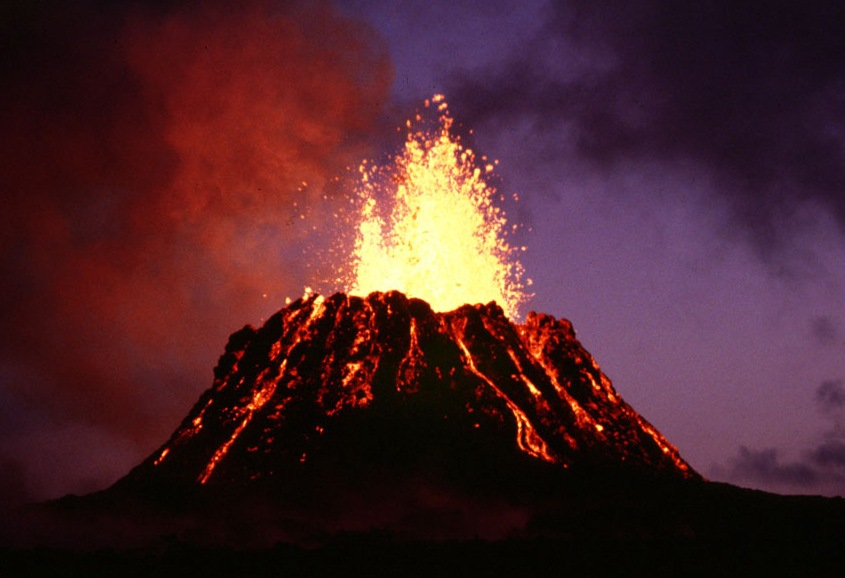
\includegraphics[width=0.55\linewidth]{images/book3/b1-puu-oo-1983.jpg}
\par\smallskip{\small Pu\textquoteleft u~\textquoteleft O\textquoteleft o शंकु पर एक लावा-फ़व्वारा, किलाउआ के पूर्वी दरार-क्षेत्र पर, 29 जून 1983 को, दशकों तक चले उद्गार के पहले वर्ष में: गरम और तरल बेसाल्टिक लावा, एक धारा में ऊपर फेंका जाता और छिद्र के चारों ओर वापस गिरता हुआ। चित्र: G.~E.~Ulrich, U.S. Geological Survey, सार्वजनिक डोमेन (Wikimedia Commons)।}
\label{fig:b1:hotspots:puu-oo}
\end{omfigure}
% ledger: commons:puu-oo, pp1801:kilauea-rate

\begin{history}[प्लेटों के लिए एक स्थिर चौखटा]
1963 में जॉन टूज़ो विल्सन ने हवाई द्वीपों को, जो एक रेखा के साथ अधिकाधिक पुराने हैं, प्रावार-संवहन कोष्ठ के धीमे कोर में रखे लावा के एक स्रोत से समझाया, जबकि कोष्ठ का तेज़ ऊपरी भाग समुद्र-तल को उसके ऊपर से ले जाता था। 1971 और 1972 में डब्ल्यू॰ जेसन मॉर्गन ने उस स्रोत को एक स्तंभ बनाया, लगभग \qty{150}{km} आर-पार, जो \omterm{def:b1:layered-earth:layers}{प्रावार} के निचले भाग से उठता है और इसलिए उसके ऊपर प्लेटों के चलने पर लगभग स्थिर रहता है; टंकी-प्रयोगों ने शीघ्र ही दिखाया कि ऐसा स्तंभ कैसा दिखता है। \omterm{def:b1:hotspots:hotspot}{हॉटस्पॉट} एक ऐसा चौखटा बन गए जिसमें प्लेटों को केवल एक-दूसरे के सापेक्ष नहीं, \omterm{def:b1:layered-earth:layers}{प्रावार} के सापेक्ष मापा जा सका। आधी सदी बाद पता चला है कि यह चौखटा खिसकता है, हवाई \omterm{def:b1:hotspots:hotspot}{हॉटस्पॉट} उनमें से एक है, पर इतनी धीमी गति से कि प्रशांत पथ अब भी \omterm{def:b1:layered-earth:layers}{प्रावार} के ऊपर प्लेट की गति प्रति वर्ष कुछ अंशों और कुछ सेंटीमीटर तक दे देते हैं, जैसा इस अध्याय के फ़िट ने दिखाया।
\end{history}
% ledger: hist:plumes, tarduno:emperor

\section{बृहत आग्नेय प्रांत}\label{sec:b1:hotspots:lips}

\begin{definition}[बृहत आग्नेय प्रांत]
\label{def:b1:hotspots:lip}
\emph{बृहत आग्नेय प्रांत}\index{बृहत आग्नेय प्रांत} (LIP) आग्नेय चट्टान का एक संचय है, अधिकतर बेसाल्ट, जो कटक पर साधारण प्रसार से नहीं बनता, \qty{e5}{km^2} से अधिक क्षेत्र घेरता है, \qty{e5}{km^3} से अधिक धारण करता है, और अधिकतम लगभग 50 मिलियन वर्षों के भीतर स्थापित हुआ, जिसका अधिकांश 1 से 5 मिलियन वर्ष की स्पंदों में, जो उसके आयतन के तीन-चौथाई से अधिक वहन करते हैं। स्थल पर LIP अधिकतर बाढ़-बेसाल्ट हैं; महासागरों में, महासागरीय पठार।
\end{definition}

एक विशिष्ट LIP लगभग दस लाख वर्ग किलोमीटर घेरता है और लगभग दस लाख घन किलोमीटर लावा धारण करता है, जिसका अधिकांश लगभग दस लाख वर्ष या उससे कम में उगला गया। उनके लावा लगभग समतल प्रवाहों में ढेर होते हैं, जिन्हें अपरदन सीढ़ियों में काटता है, उनके नामों के \emph{ट्रैप्स}। सारणी पिछले 260 मिलियन वर्षों के मुख्य प्रांत सूचीबद्ध करती है।
% ledger: be08:definition, cr03:summary

\begin{omfigure}
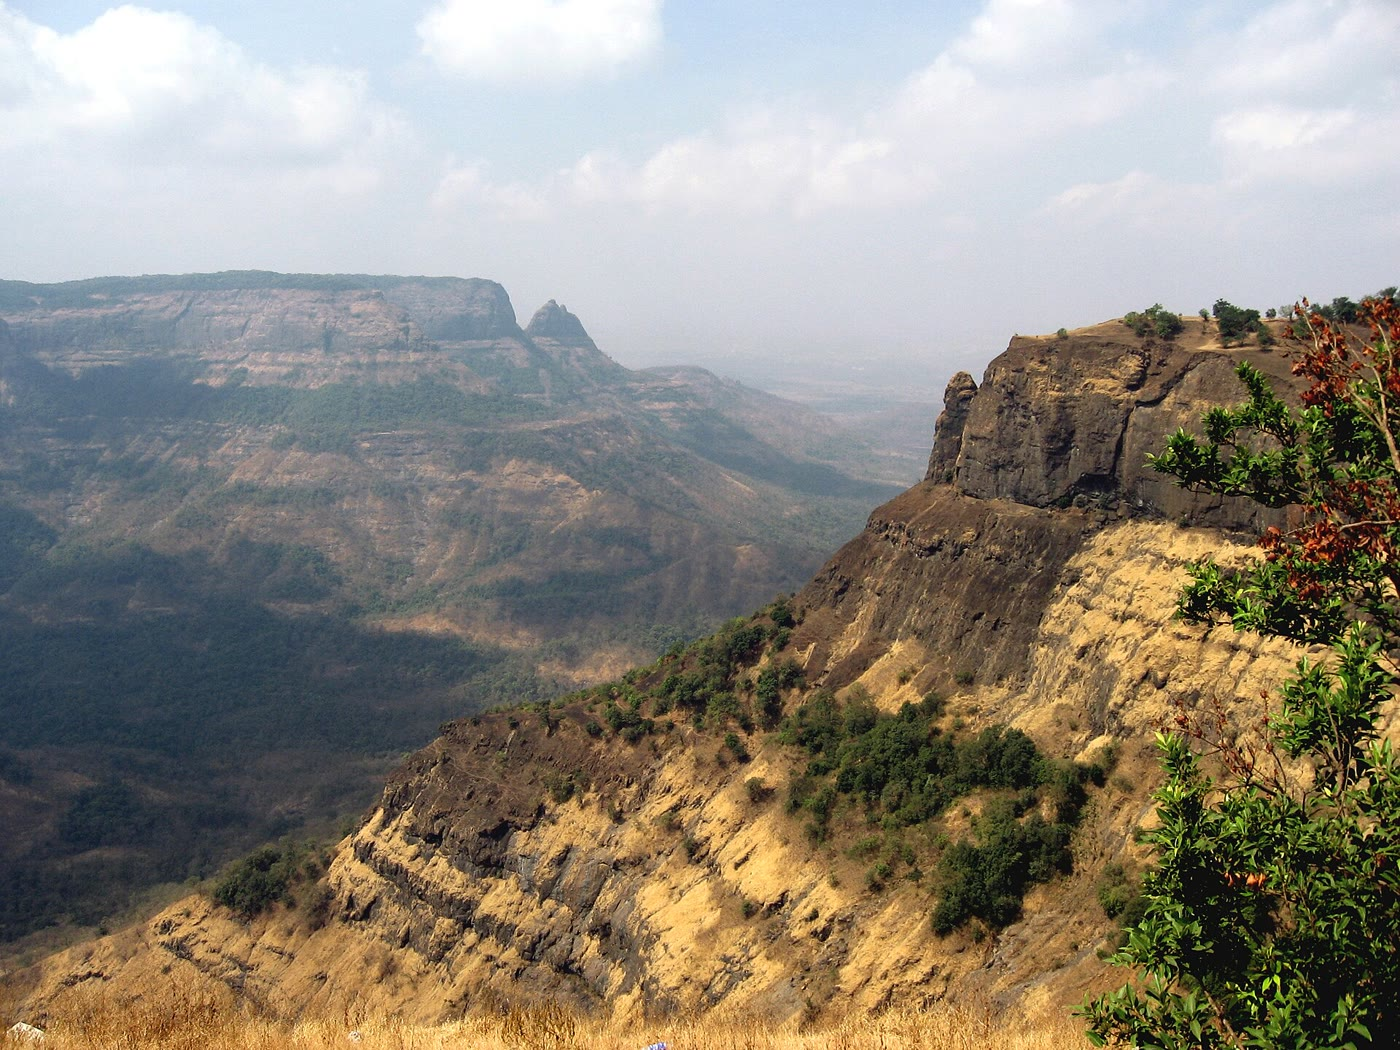
\includegraphics[width=0.55\linewidth]{images/book3/b1-deccan-matheran.jpg}
\par\smallskip{\small भारत में माथेरान के निकट पश्चिमी घाट: समतल-शीर्ष पहाड़ियाँ, जो डेक्कन ट्रैप्स के लगभग क्षैतिज लावा-प्रवाहों के ढेर में कटी हैं, जिनकी प्रतिरोधी परतें ढलानों की सीढ़ियाँ बनाती हैं। चित्र: Nicholas (Nichalp), CC BY-SA 2.5 (Wikimedia Commons)।}
\label{fig:b1:hotspots:deccan}
\end{omfigure}
% ledger: commons:matheran

\begin{center}
\small
\begin{tabular}{llll}
\hline
प्रांत & आयु (Ma) & क्षेत्रफल (\unit{Mkm^2}) & पहला आयतन (\unit{Mkm^3})\\
\hline
कोलंबिया नदी & 16 & 0.2 & 0.2\\
इथियोपिया–यमन & 30 & 0.7 & 1.2\\
उत्तर अटलांटिक & 61 और 56 & 1.2 & 2 से अधिक\\
डेक्कन & 65.5 & 0.5 (एक बार 1.8) & 2 से 4\\
ओंटोंग जावा & 122 और 90 & 2 & 44 (पूरी \omterm{def:b1:layered-earth:layers}{भूपर्पटी})\\
पारानी–एटेंडेका & 133 & 1.5 (एक बार 2 से अधिक) & 2.3 से अधिक\\
कारू–फेरार & 183 & 3.1 & 2.5 से अधिक\\
मध्य अटलांटिक (CAMP) & 201 & एक बार 7 तक & 2 से अधिक\\
साइबेरियाई ट्रैप्स & 250 & 0.4 (एक बार 4 से अधिक) & 3 से अधिक\\
एमेइशान & 259 & 0.5 (एक बार 2 से 5) & 1 से अधिक\\
\hline
\end{tabular}
\par\smallskip{\small औसत आयु; क्षेत्रफल जैसे वे आज हैं, और जैसे वे पहली बार उगले गए जहाँ अनुमान उपलब्ध है; लावा के आयतन जैसे पहली बार उगले गए, ओंटोंग जावा पठार को छोड़कर, जिसका आँकड़ा उसकी पूरी मोटी हुई \omterm{def:b1:layered-earth:layers}{भूपर्पटी} गिनता है। आँकड़े: वी॰~कुर्तियो और पी॰~रेन (2003)।}
\end{center}
% ledger: cr03:table

\noindent \cref{sec:b1:hotspots:plumes} में खींचा गया \omterm{def:b1:hotspots:plume}{प्रावार-स्तंभ} मॉडल आकार और तीव्रता दोनों समझाता है: सैकड़ों किलोमीटर आर-पार का एक स्तंभ-शीर्ष \omterm{def:b1:layered-earth:lithosphere}{स्थलमंडल} के आधार तक पहुँचता है, दाब घटाता है और पिघलता है, और सतह को प्लावित करता है; फिर पुच्छ एक साधारण \omterm{def:b1:hotspots:track}{हॉटस्पॉट-पथ} बनाती रहती है। कई प्रांत एक जीवित पथ के पुराने छोर पर खड़े माने जाते हैं: डेक्कन ट्रैप्स और रेयूनियन \omterm{def:b1:hotspots:hotspot}{हॉटस्पॉट}, पारानी–एटेंडेका और ट्रिस्टन दा कुन्हा, जिन्हें वॉलविस कटक जोड़ता है, और कोलंबिया नदी के बेसाल्ट और येलोस्टोन।
% ledger: cr03:deccan (Reunion hot spot, plume-head model), be08:ojmh (Parana-Etendeka-Walvis-Tristan), pm90:track (Columbia River basalts)

पश्चिम-मध्य भारत के डेक्कन ट्रैप्स लावा-प्रवाहों का एक ढेर हैं, लगभग \qty{2500}{m} मोटा, जिसका कम से कम \qty{1800}{m} 65.5 मिलियन वर्ष पहले के निकट, दस लाख वर्ष से बहुत कम में उगला गया; आज वे लगभग \qty{0.5}{\mega km^2} ढकते हैं, अपरदन से पहले शायद \qty{1.8}{\mega km^2}। दक्षिण-पश्चिम प्रशांत का ओंटोंग जावा पठार सभी महासागरीय पठारों में सबसे बड़ा है: वह लगभग \qty{2}{\mega km^2} ढकता है, और उसकी \omterm{def:b1:layered-earth:layers}{भूपर्पटी}, लगभग \qty{36}{km} मोटी, लगभग \qty{44}{\mega km^3} आग्नेय चट्टान धारण करती है। मनिहिकी और हिकुरांगी पठार, जो अब नए महासागर-तल से पार उससे दूर हैं, शायद उसके साथ एक ही पठार के रूप में बने थे। मध्य अटलांटिक मैग्मा प्रांत, जो लगभग 201 मिलियन वर्ष पहले उगला गया जब अटलांटिक खुलने लगा, आज लावाओं, डाइकों और सिलों के रूप में चार महाद्वीपों में बिखरा है: पूर्वी उत्तर अमेरिका, उत्तर-पूर्वी दक्षिण अमेरिका, पश्चिम अफ़्रीका और दक्षिण-पश्चिम यूरोप; वह कभी \qty{7}{\mega km^2} तक ढक सकता था।
% ledger: cr03:deccan, cr03:table, cr03:ontong-java, be08:ojmh, cr03:camp


कई प्रांत उन महान सामूहिक विलोपनों के साथ समय में संपाती हैं जिन्हें जीवविज्ञान वर्णित करता है: साइबेरियाई ट्रैप्स सभी में सबसे बड़े विलोपन के साथ, पर्मियन के अंत में; मध्य अटलांटिक प्रांत ट्राइऐसिक के अंत के साथ; कारू–फेरार प्रारंभिक जुरासिक के एक विलोपन के साथ; एमेइशान मध्य पर्मियन के एक विलोपन के साथ; और डेक्कन ट्रैप्स क्रिटेशस के अंत के साथ। पिछले 260 मिलियन वर्षों के चार सबसे बड़े विलोपनों में से हर एक, तिथियाँ जितने निकटता से बता सकती हैं, इन प्रांतों में से किसी एक पर पड़ता है, और कारणात्मक संबंध सबसे संभावित माना जाता है। प्रस्तावित तंत्र वायुमंडलीय हैं: सल्फेट एरोसोल जो थोड़े समय के लिए जलवायु को ठंडा करते हैं, कार्बन डाइऑक्साइड जो उसे बहुत लंबे समय तक गरम करती है, और ऑक्सीजन से वंचित महासागर। क्रिटेशस के अंत के लिए, डेक्कन उद्गार चिक्सुलब पर प्रभाव से पहले शुरू हुए और उसके बाद भी चलते रहे; सीमा के अभिलेखों की एक समीक्षा ने 2010 में निष्कर्ष निकाला कि प्रभाव ने विलोपन को उत्प्रेरित किया।
% ledger: cr03:table, cr03:summary, cr03:deccan, schulte:kpg

प्लेट-सीमाओं से दूर का हर ज्वालामुखी-क्रियाकलाप स्तंभ नहीं माँगता। छोटे ज्वालामुखी-क्षेत्र वहाँ बनते हैं जहाँ कोई प्लेट खिंचती या दरकती है, और जिन शृंखलाओं में स्पष्ट \omterm{def:b1:hotspots:track}{आयु-प्रगति} नहीं है वे ऊपरी \omterm{def:b1:layered-earth:layers}{प्रावार} से पोषित हो सकती हैं; यह प्लेट-परिकल्पना का काम है। \omterm{def:b1:hotspots:hotspot}{हॉटस्पॉट} द्वारा छोड़ने के बाद महासागरीय द्वीप क्या बनते हैं, जब वे धँसते हैं, घिसते हैं और प्रवाल-भित्तियाँ उगाते हैं, वह पुस्तक 4 का विषय है।
% ledger: fn03:plate-hypothesis

\section{अभ्यास}

\begin{exercise}[$\star$]\label{exo:b1:hotspots:1}
(क) माउना केआ समुद्र-तल से \qty{4205}{m} ऊपर उठता है, और हवाई शृंखला से दूर का समुद्र-तल \qty{5274}{m} गहरा है। ज्वालामुखी उस तल से कितना ऊँचा खड़ा है? उसके आधार से वास्तविक ऊँचाई फिर भी बड़ी क्यों है? (ख) माउना लोआ लगभग \qty{74000}{km^3} धारण करता है। किलाउआ की वर्तमान आपूर्ति, \qty{0.1}{km^3} प्रति वर्ष, पर, और पूरी शृंखला की औसत दर, \qty{0.025}{km^3} प्रति वर्ष पर, उसे बनाने में कितना समय लगेगा? (ग) Pu\textquoteleft u~\textquoteleft O\textquoteleft o का उद्गार 1983 से 2002 तक लगभग \qty{0.12}{km^3} प्रति वर्ष उगलता रहा। वह कितना आयतन है, और माउना लोआ का कितना अंश?
% ledger: pp1801:volumes, pp1801:kilauea-supply, pp1801:chain-volume, pp1801:kilauea-rate; 5274 m from hotspots.py
\end{exercise}

\begin{exercise}[$\star$]\label{exo:b1:hotspots:2}
एक प्लेट हॉटस्पॉटों के ऊपर \qty{0.92}{\degree\per\Myr} पर घूमती है। लीजिए $R = \qty{6371}{km}$। (क) $\omega$ को रेडियन प्रति मिलियन वर्ष में व्यक्त कीजिए। (ख) \unit{mm.yr^{-1}} में, ध्रुव से \ang{30}, \ang{60}, \ang{90} और \ang{108.0} पर स्थित हॉटस्पॉटों की चाल परिकलित कीजिए। (ग) \ang{108.0} पर स्थित हवाई की चाल \ang{90} से कम क्यों है?
\end{exercise}

\begin{exercise}[$\star$]\label{exo:b1:hotspots:3}
(क) डेक्कन ट्रैप्स की आज की औसत मोटाई परिकलित कीजिए, \qty{0.5}{\mega km^2} पर \qty{1}{\mega km^3}, और मध्य अटलांटिक प्रांत की, \qty{7}{\mega km^2} पर \qty{2}{\mega km^3}। (ख) उसकी तुलना डेक्कन खंड की मोटाई, \qty{2500}{m}, से कीजिए। (ग) मध्य अटलांटिक प्रांत की औसत मोटाई उसके लावा-ढेरों की मोटाई के बारे में कम क्यों कहती है?
% ledger: cr03:table, cr03:deccan, cr03:camp
\end{exercise}

\begin{exercise}[$\star$]\label{exo:b1:hotspots:4}
आसपास के \omterm{def:b1:layered-earth:layers}{प्रावार} से \qty{250}{K} गरम स्तंभ-चट्टान की $\alpha = \qty{3.2e-5}{K^{-1}}$ और $\rho_m = \qty{3300}{kg.m^{-3}}$ है। (क) \unit{kg.m^{-3}} में वह कितनी हल्की है? (ख) प्लेट के नीचे फैली ऐसी चट्टान की कितनी मोटाई समुद्र के नीचे \qty{690}{m} ऊँचे उभार को समस्थितिक रूप से टिका सकेगी ($\rho_w = \qty{1000}{kg.m^{-3}}$)?
% ledger: herzberg:tp (200-300 K), parsons:plate-model (alpha)
\end{exercise}

\begin{exercise}[$\star\star$]\label{exo:b1:hotspots:5}
दो \omterm{def:b1:hotspots:hotspot}{हॉटस्पॉट} भूमध्य-रेखा पर हैं, A \ang{0}\,E पर और B \ang{90}\,E पर, और दोनों पथ ठीक पश्चिम चलते हैं (दिगंश \ang{270})। (क) पथ-सदिश $\vec t_A$ और $\vec t_B$ परिकलित कीजिए। (ख) $\vec t_A\times\vec t_B$ परिकलित कीजिए। (ग) \cref{prop:b1:hotspots:two-tracks} का चिह्न-नियम लगाइए: \omterm{def:b1:plate-kinematics:euler-pole}{यूलर ध्रुव} कहाँ है? परिकलन के बिना परिणाम समझाइए। (घ) यदि A \qty{50}{mm.yr^{-1}} से चलता है, तो $\omega$ प्रति मिलियन वर्ष कितने अंश में है?
\end{exercise}

\begin{exercise}[$\star\star$]\label{exo:b1:hotspots:6}
एक प्लेट के तीन \omterm{def:b1:hotspots:hotspot}{हॉटस्पॉट} परिभ्रमण-अक्ष से $x = R\sin\Delta = 3000$, 5000 और \qty{6000}{km} दूरियों पर पड़ते हैं और 30, 48 और \qty{57}{mm.yr^{-1}} से चलते हैं। (क) न्यूनतम-वर्ग से $v = \omega x$ फ़िट कीजिए और $\omega$ रेडियन में और प्रति मिलियन वर्ष अंशों में दीजिए। (ख) अवशेष परिकलित कीजिए। (ग) रेखा मूलबिंदु से होकर क्यों जानी चाहिए?
\end{exercise}

\begin{exercise}[$\star\star$]\label{exo:b1:hotspots:7}
\qty{3e8}{m^2} अनुप्रस्थ-काट का एक उभार \qty{50}{mm.yr^{-1}} से चलती प्लेट पर एक \omterm{def:b1:hotspots:track}{हॉटस्पॉट-पथ} को घेरता है। लीजिए $\rho_m - \rho_w = \qty{2300}{kg.m^{-3}}$, $c_p = \qty{910}{J.kg^{-1}.K^{-1}}$ और $\alpha = \qty{3.2e-5}{K^{-1}}$। (क) उसका उत्प्लावकता-प्रवाह और उसका \omterm{def:b1:heat-budget:heat-flow}{ऊष्मा-प्रवाह} परिकलित कीजिए। (ख) हवाई, \qty{3240}{kg.s^{-1}}, से तुलना कीजिए। (ग) दो हॉटस्पॉटों का उभार एक-सा है; एक ऐसी प्लेट के नीचे है जो दोगुनी तेज़ चलती है। कौन-सा स्तंभ प्रबलतर है?
\end{exercise}

\begin{exercise}[$\star\star$]\label{exo:b1:hotspots:8}
येलोस्टोन पथ के साथ, कैल्डेरा-उद्गार 16.1 मिलियन वर्ष पहले मैकडर्मिट ज्वालामुखी-क्षेत्र में, और लगभग \qty{350}{km} उत्तर-पूर्व में स्थित पिकाबो क्षेत्र में 10.3 मिलियन वर्ष पहले शुरू हुए; तब से वे $\qty[uncertainty-mode=separate]{2.9 \pm 0.5}{cm}$ प्रति वर्ष की दर से N\,\ang{54}\,E की ओर खिसके हैं। (क) ज्वालामुखी-क्रिया किस औसत चाल से मैकडर्मिट से पिकाबो तक खिसकी? (ख) दोनों चालों की तुलना \omterm{def:b1:hotspots:hotspot}{हॉटस्पॉट} के ऊपर प्लेट की चाल से कीजिए, \qty[uncertainty-mode=separate]{26 \pm 5}{mm.yr^{-1}}, \ang{235} की ओर। (ग) क्या युवा पथ की दिशा वही है जिसकी अपेक्षा थी? (घ) पथ का पुराना भाग एक ऐसे क्षेत्र में पड़ता है जो ज्वालामुखी-क्रिया के गुज़रने के साथ खिंचा गया है। यह अंतर कैसे समझा सकता है?
% ledger: pm90:track, data:b3-hotspots
\end{exercise}

\begin{exercise}[$\star\star$]\label{exo:b1:hotspots:9}
हवाई स्तंभ लगभग \qty{9.2e10}{W} अतिरिक्त ऊष्मा वाहित करता है। (क) यदि उसका सब कुछ \omterm{def:b1:hotspots:hotspot}{हॉटस्पॉट} के निकटतम \qty{1000}{km} गुणा \qty{1000}{km} समुद्र-तल से निकले, तो वहाँ का \omterm{def:b1:heat-budget:heat-flow}{ऊष्मा-प्रवाह} कितना बढ़ेगा? (ख) उसकी तुलना प्रेक्षित अतिरिक्त से कीजिए, अधिकतम 5 से \qty{10}{mW.m^{-2}}। (ग) \qty{100}{km} मोटी प्लेट के आर-पार ऊष्मा को विसरित होने में कितना समय लगता है ($\kappa = \qty{e-6}{m^2.s^{-1}}$)? \qty{92}{mm.yr^{-1}} पर प्लेट को \qty{1000}{km} पार करने में कितना समय लगता है? निष्कर्ष निकालिए।
% ledger: vh89:swell-heat
\end{exercise}

\begin{exercise}[$\star\star\star$]\label{exo:b1:hotspots:10}
डेक्कन ट्रैप्स में लगभग \qty{e6}{km^3} लावा है। मान लीजिए वह एक गोलाकार स्तंभ-शीर्ष से आया, जिसका दसवाँ भाग पिघला। (क) शीर्ष का आयतन और त्रिज्या क्या थी? (ख) \omterm{def:b1:layered-earth:lithosphere}{स्थलमंडल} के नीचे \qty{100}{km} मोटी एक चकती में चपटा होने पर, शीर्ष का व्यास क्या होता? उसके क्षेत्रफल की तुलना उस क्षेत्रफल से कीजिए जिसे ट्रैप्स कभी ढकते थे, \qty{1.8}{\mega km^2}। (ग) यदि लावा दस लाख वर्ष में उगला गया, तो उसकी दर की तुलना किलाउआ की वर्तमान आपूर्ति, \qty{0.1}{km^3} प्रति वर्ष, से कीजिए। (घ) स्तंभ-शीर्ष बड़ा क्यों होना चाहिए, जबकि उसके बाद आने वाली पुच्छ संकरी है?
% ledger: cr03:table, pp1801:kilauea-supply
\end{exercise}

\begin{exercise}[$\star\star\star$]\label{exo:b1:hotspots:11}
81 से 47 मिलियन वर्ष पहले हवाई \omterm{def:b1:hotspots:hotspot}{हॉटस्पॉट} \qty{40}{mm.yr^{-1}} से अधिक चाल से दक्षिण की ओर खिसका। (क) \qty{40}{mm.yr^{-1}} लेकर, वह कितनी दूर खिसका? (ख) मान लीजिए इस बीच प्लेट गहरे \omterm{def:b1:layered-earth:layers}{प्रावार} के ऊपर \ang{340} की ओर \qty{80}{mm.yr^{-1}} से चली। $x$ पूर्व और $y$ उत्तर मानकर, खिसकते \omterm{def:b1:hotspots:hotspot}{हॉटस्पॉट} के सापेक्ष प्लेट का वेग, उसकी चाल और उसका दिगंश परिकलित कीजिए। (ग) उस समय बना पथ गहरे \omterm{def:b1:layered-earth:layers}{प्रावार} के ऊपर प्लेट की गति को कितने प्रतिशत, और कितने अंश, गलत दर्शाता?
% ledger: tarduno:emperor
\end{exercise}

\begin{exercise}[$\star\star\star$]\label{exo:b1:hotspots:12}
(क) एक बाढ़-बेसाल्ट, \qty{e6}{km^3}, लगभग \qty{1300}{\celsius} से सतह के तापमान तक ठंडा होता है। \qty{3}{MJ.m^{-3}.K^{-1}} की ऊष्मा-धारिता के साथ, वह कितनी ऊष्मा निकालता है (क्रिस्टलीकरण की गुप्त ऊष्मा उपेक्षित कीजिए)? (ख) दस लाख वर्ष पर फैलाने पर वह कितनी शक्ति है? उसकी तुलना हवाई स्तंभ, \qty{9.2e10}{W}, और पूरी पृथ्वी की \qty{47}{TW} से कीजिए। (ग) स्तंभ-शीर्ष \omterm{def:b1:layered-earth:lithosphere}{स्थलमंडल} के आधार को भी बिना पूरा पिघलाए गरम करता है। क्या (ख) की शक्ति स्तंभ-शीर्ष द्वारा लाई गई ऊष्मा की ऊपरी सीमा है या निचली सीमा?
% ledger: delaney86:properties (Book 2 row, 2-3 MJ/m3/K), dd10:total; 1300 degC is an exercise value
\end{exercise}

\section{समस्या: प्रशांत प्लेट का गति-मापी}

\begin{problem}[{सप्ताहांत समस्या --- दो हॉटस्पॉट-पथों से प्रशांत प्लेट का यूलर ध्रुव, एक तीसरे माप से उसकी दर, अन्य हॉटस्पॉटों पर एक परीक्षा, और हवाई स्तंभ की उत्प्लावकता और आपूर्ति}]
\label{pb:b1:hotspots:1}
% values: calc/ch15.py; ledger: data:b3-hotspots, data:etopo1, pp1801:kilauea-supply, pp1801:volumes,
% pp1801:chain-volume, delaney86:properties, parsons:plate-model, dd10:total, data:pb2002 (ridge_budget.py), cd87:rate
मॉर्गन और मॉर्गन हवाई \omterm{def:b1:hotspots:hotspot}{हॉटस्पॉट} को \ang{19.0}\,N, \ang{155.2}\,W पर रखते हैं, जिसका पथ $\ang{304}\pm\ang{3}$ की ओर और चाल \qty[uncertainty-mode=separate]{92 \pm 3}{mm.yr^{-1}} है, और लुईसविल \omterm{def:b1:hotspots:hotspot}{हॉटस्पॉट} \ang{53.6}\,S, \ang{140.6}\,W पर, जिसका पथ $\ang{316}\pm\ang{5}$ की ओर और चाल \qty[uncertainty-mode=separate]{67 \pm 5}{mm.yr^{-1}} है। अक्षों और सदिशों $\vec e$, $\vec n$, $\vec t$ का प्रयोग कीजिए जो \cref{sec:b1:hotspots:tracks} में हैं, $R = \qty{6371}{km}$ के साथ। घटक चार दशमलव तक दीजिए।

\medskip
\noindent\textbf{भाग I --- दो पथों से ध्रुव।}
\begin{enumerate}
  \item हवाई पर $\vec r$, $\vec e$ और $\vec n$ परिकलित कीजिए, फिर पथ-सदिश $\vec t_H$।
  \item उसी प्रकार लुईसविल पर: $\vec r_L$, $\vec e$, $\vec n$ और $\vec t_L$।
  \item जाँचिए कि $\vec t_H$ एक इकाई सदिश है जो $\vec r_H$ के लंबवत है।
  \item $\vec t_H\times\vec t_L$ और उसकी लंबाई परिकलित कीजिए। दोनों पथ-सदिश किस कोण पर हैं?
  \item सदिश गुणनफल को इकाई बनाइए और \cref{prop:b1:hotspots:two-tracks} का चिह्न-नियम लगाइए।
  \item हॉटस्पॉटों के सापेक्ष प्रशांत प्लेट के \omterm{def:b1:plate-kinematics:euler-pole}{यूलर ध्रुव} का \omterm{def:b1:spherical-astronomy:geographic}{अक्षांश} और \omterm{def:b1:spherical-astronomy:geographic}{देशांतर} दीजिए।
\end{enumerate}

\medskip
\noindent\textbf{भाग II --- दर।}
\begin{enumerate}[resume]
  \item दोनों हॉटस्पॉटों तक ध्रुव से कोणीय दूरियाँ $\Delta_H$ और $\Delta_L$ परिकलित कीजिए।
  \item $(\vec p\times\vec r_L)\cdot\vec t_L$ परिकलित कीजिए। समझाइए कि वह क्यों $\sin\Delta_L$ के बराबर है, और उसका चिह्न लुईसविल पर की गति के बारे में क्या कहता है।
  \item लुईसविल की चाल से $\omega$ रेडियन में और प्रति मिलियन वर्ष अंशों में परिकलित कीजिए।
  \item प्रशांत प्लेट को इस ध्रुव के परितः एक पूरा चक्कर लगाने में कितना समय लगता है?
  \item प्रशांत के पंद्रह पथों का न्यूनतम-वर्ग ध्रुव \ang{63.78}\,S, \ang{112.48}\,E पर है, \qty{0.92}{\degree\per\Myr} के साथ। दोनों ध्रुवों के बीच का कोण परिकलित कीजिए और दोनों दरों की तुलना कीजिए।
\end{enumerate}

\medskip
\noindent\textbf{भाग III --- तीन और हॉटस्पॉटों पर एक परीक्षा।} मॉर्गन और मॉर्गन सोसाइटी \omterm{def:b1:hotspots:hotspot}{हॉटस्पॉट} (\ang{18.2}\,S, \ang{148.4}\,W) को \qty[uncertainty-mode=separate]{109 \pm 10}{mm.yr^{-1}}, पिटकेर्न (\ang{25.4}\,S, \ang{129.3}\,W) को \qty[uncertainty-mode=separate]{90 \pm 15}{mm.yr^{-1}} और कॉब (\ang{46.0}\,N, \ang{130.1}\,W) को \qty[uncertainty-mode=separate]{43 \pm 3}{mm.yr^{-1}} देते हैं।
\begin{enumerate}[resume]
  \item प्रश्न 6 के ध्रुव से तीनों हॉटस्पॉटों में से हर एक तक कोणीय दूरी परिकलित कीजिए।
  \item प्रश्न 9 की दर से तीन चालों का पूर्वानुमान कीजिए।
  \item कौन-से पूर्वानुमान अपनी अनिश्चितताओं के भीतर मापी गई चालों से मेल खाते हैं, और कौन-से नहीं?
  \item दो भिन्न दिशाओं वाले पथ सदैव एक ध्रुव देते हैं। लगभग समांतर दो पथ एक खराब चुनाव क्यों हैं?
\end{enumerate}

\medskip
\noindent\textbf{भाग IV --- स्तंभ और गति-मापी।} हवाई उभार का अनुप्रस्थ-काट \qty{4.83e8}{m^2} है। लीजिए $\rho_m - \rho_w = \qty{2300}{kg.m^{-3}}$, $c_p = \qty{910}{J.kg^{-1}.K^{-1}}$ और $\alpha = \qty{3.2e-5}{K^{-1}}$।
\begin{enumerate}[resume]
  \item \qty{92}{mm.yr^{-1}} को \unit{m.s^{-1}} में बदलिए और हवाई स्तंभ का उत्प्लावकता-प्रवाह परिकलित कीजिए।
  \item वह अतिरिक्त ऊष्मा परिकलित कीजिए जो वह वाहित करता है, और उसकी तुलना पृथ्वी से निकलने वाली \qty{47}{TW} से कीजिए।
  \item कटक कुछ \qty{67000}{km} लंबाई पर प्रति वर्ष लगभग \qty{21}{km^3} \omterm{def:b1:layered-earth:layers}{भूपर्पटी} बनाते हैं। कटक की कितनी लंबाई उतनी \omterm{def:b1:layered-earth:layers}{भूपर्पटी} बनाती है जितनी किलाउआ को प्रति वर्ष \qty{0.1}{km^3} आपूर्ति मिलती है?
  \item इस दर से, माउना लोआ, लगभग \qty{74000}{km^3}, को बढ़ने में कितना समय लगेगा?
  \item \omterm{def:b1:hotspots:hotspot}{हॉटस्पॉट} ने 81 मिलियन वर्ष में शृंखला का लगभग \qty{2e6}{km^3} बनाया। उसका औसत उत्पादन परिकलित कीजिए और आज की किलाउआ की आपूर्ति से तुलना कीजिए।
  \item भाग I और II के ध्रुव और दर के साथ, वह चाल परिकलित कीजिए जो लुईसविल पथ हवाई \omterm{def:b1:hotspots:hotspot}{हॉटस्पॉट} के ऊपर प्रशांत प्लेट के लिए अनुमानित करता है।
  \item मापी गई \qty[uncertainty-mode=separate]{92 \pm 3}{mm.yr^{-1}} से तुलना कीजिए: वे कितना, और कितने मानक अनिश्चितता-गुणकों से, भिन्न हैं?
  \item हवाई ज्वालामुखियों की आयुओं से पुस्तक 2 ने \qty{9.1}{cm} प्रति वर्ष पाया, और आयुओं के लेखकों ने, पूरी शृंखला को फ़िट करते हुए, \qty{8.6}{cm} प्रति वर्ष। दसियों मिलियन वर्षों पर इन औसतों की दोनों हॉटस्पॉट-चालों से तुलना कीजिए।
  \item सेंटीमीटर प्रति वर्ष में एक दशमलव तक, लुईसविल पथ प्रशांत प्लेट को हवाई \omterm{def:b1:hotspots:hotspot}{हॉटस्पॉट} के ऊपर कौन-सी चाल देता है?
\end{enumerate}
\end{problem}
